\documentclass[11pt,a4paper]{article}
\usepackage[utf8]{inputenc}
\usepackage[T1]{fontenc}
\usepackage{lmodern}
% Idioma: usa el módulo español de babel si está instalado; si no, traduce los nombres a mano.
\IfFileExists{spanish.ldf}{%
  \usepackage[spanish,es-noshorthands,es-tabla]{babel}%
}{%
  \usepackage[english]{babel}%
  \addto\captionsenglish{%
    \renewcommand{\abstractname}{Resumen}%
    \renewcommand{\figurename}{Figura}%
    \renewcommand{\tablename}{Tabla}%
    \renewcommand{\refname}{Referencias}%
    \renewcommand{\contentsname}{Contenido}%
    \renewcommand{\appendixname}{Apéndice}%
  }%
  \renewcommand{\today}{15 de octubre de 2026}%
}
\usepackage{amsmath, amssymb, bm}
\usepackage[a4paper, left=2.5cm, right=2.5cm, top=2.8cm, bottom=2.8cm]{geometry}
\usepackage{graphicx}
\usepackage{booktabs}
\usepackage{tabularx}
\usepackage{subcaption}
\usepackage[font=small, labelfont=bf]{caption}
\usepackage{microtype}
\usepackage{xcolor}
\usepackage[separate-uncertainty=true, group-separator={\,}, group-minimum-digits=4]{siunitx}
\usepackage[colorlinks=true, linkcolor=blue!50!black, citecolor=blue!50!black, urlcolor=blue!50!black]{hyperref}

\graphicspath{{figures/}}
% Archivo autogenerado por scripts/generate_figures.py. NO EDITAR A MANO.
\newcommand{\RLiftoffMassT}{2\,710}
\newcommand{\RSrbScale}{1.0033}
\newcommand{\RTMachOneS}{52.3}
\newcommand{\RHMachOneKm}{7.3}
\newcommand{\RTMaxqS}{64.8}
\newcommand{\RMaxqKpa}{27.5}
\newcommand{\RHMaxqKm}{11.8}
\newcommand{\RMachMaxq}{1.43}
\newcommand{\RTSrbSepS}{126}
\newcommand{\RHSrbSepKm}{56.9}
\newcommand{\RVSrbSepKms}{1.43}
\newcommand{\RTMecoS}{480.5}
\newcommand{\RHMecoKm}{160.0}
\newcommand{\RVMecoKms}{6.596}
\newcommand{\RFpaMecoDeg}{0.00}
\newcommand{\RDownrangeMecoKm}{980}
\newcommand{\RMaxG}{3.50}
\newcommand{\RVCircMecoKms}{7.808}
\newcommand{\RMassMecoT}{265.3}
\newcommand{\REusPayloadT}{37.4}
\newcommand{\RDvInsertionKms}{1.212}
\newcommand{\RDvEusTotalKms}{5.547}
\newcommand{\RVerletMaxDe}{\num{1.5e-4}}
\newcommand{\RRkFourFinalDe}{\num{3.4e-3}}
\newcommand{\RDopEightFiveThreeFinalDe}{\num{6.7e-10}}
\newcommand{\RVerletMaxDh}{\num{1.2e-14}}
\newcommand{\RNOrbitsCmp}{200}
\newcommand{\RStepsPerOrbitCmp}{40}
\newcommand{\ROrderVerlet}{2.00}
\newcommand{\ROrderRkFour}{4.14}
\newcommand{\RHParkKm}{160}
\newcommand{\RTliDvMs}{3\,150.2}
\newcommand{\RTliGuessDvMs}{3\,146.4}
\newcommand{\RTliIterations}{5}
\newcommand{\RTliFinalResidualM}{\num{4.2e-4}}
\newcommand{\RTliInitialResidualKm}{23\,930}
\newcommand{\RTliFlightDays}{4}
\newcommand{\RTliFlybyAltKm}{4\,000}
\newcommand{\RTliTransferAngleDeg}{176.9}
\newcommand{\RTliApogeeKkm}{406}
\newcommand{\REusPropRemainingT}{15.8}
\newcommand{\RVerletArrivalAltKm}{4\,001}
\newcommand{\RVerletTargetMissKm}{2.37}
\newcommand{\RCondMax}{\num{2.7e4}}
\newcommand{\RJacobiMaxRel}{\num{9.7e-6}}
\newcommand{\RGeoEnergyMaxRel}{\num{7.7e-1}}


% Notación
\newcommand{\vect}[1]{\mathbf{#1}}
\newcommand{\uvec}[1]{\hat{\mathbf{#1}}}
\newcommand{\dd}{\mathrm{d}}

\title{%
\IfFileExists{logo.png}{
\includegraphics[width=3.5cm]{logo.png}\\[0.6cm]}{}%
\textbf{Simulación dinámica multifase de la misión Artemis~IV:\\ ascenso atmosférico del SLS Block~1B, integración simpléctica\\ y \emph{targeting} de la inyección translunar}}
\author{Mariana Lopera Correa \and Juan José Becerra Bedoya \and Daniel Santiago Machado\\[0.3em]
\small\textit{Programa de Computación Científica, Universidad de Medellín}}
\date{16 de octubre de 2026}

\begin{document}

\maketitle

\begin{abstract}
\noindent
Se presenta un simulador numérico en Python de las primeras fases del perfil de vuelo de la misión Artemis~IV con el lanzador \emph{Space Launch System} (SLS) Block~1B. El ascenso se modela en un marco geocéntrico inercial (ECI) como un sistema de siete ecuaciones diferenciales de primer orden con masa variable, empuje dependiente de la presión ambiental, un perfil regresivo de empuje de los propulsores sólidos (SRB) que conserva exactamente su masa de propelente, arrastre con coeficiente $C_D(M)$ y atmósfera estándar de 1976. Se integra con Dormand--Prince RK45 y detección de eventos (separación de SRB y apagado de la etapa central, MECO), con una ley de guiado de tangente lineal. El vehículo alcanza Max-Q $=\RMaxqKpa$~kPa a $t=\RTMaxqS$~s y MECO a $h=\RHMecoKm$~km con $v=\RVMecoKms$~km/s. El tránsito Tierra--Luna se formula como el Problema Restringido Circular de Tres Cuerpos, escrito en el marco geocéntrico con el término indirecto, y se integra con el esquema simpléctico Velocity Verlet, cuyo orden 2 se verifica numéricamente (pendiente $\ROrderVerlet$). En el problema de Kepler, el error de energía de Verlet permanece acotado ($\le\RVerletMaxDe$ en $\RNOrbitsCmp$ órbitas), mientras que el de RK4 con el mismo paso crece secularmente hasta $\RRkFourFinalDe$. Con la Luna, el invariante correcto es la integral de Jacobi, conservada con Verlet hasta $\RJacobiMaxRel$. Por último, la maniobra de inyección translunar (TLI) se resuelve como un problema de valores en la frontera mediante el método del disparo con Newton--Raphson, inicializado con una solución kepleriana de la ecuación de Kepler. Converge en $\RTliIterations$ iteraciones a $|\Delta\vect v|=\RTliDvMs$~m/s, consistente con el presupuesto de $\Delta v$ de la Etapa Superior de Exploración (EUS).
\end{abstract}

\tableofcontents
\newpage

%==========================================================================
\section{Introducción}
%==========================================================================
El programa Artemis de la NASA busca el retorno sostenido de seres humanos a la Luna y la construcción de la infraestructura para la exploración de Marte~\cite{nasa2020artemis}. A diferencia de las trayectorias de inyección directa del programa Apolo, la arquitectura de Artemis encadena varios regímenes orbitales y vehículos: el lanzador SLS, la cápsula Orion, la estación \emph{Gateway} en una órbita de halo casi rectilínea (NRHO) y el sistema de alunizaje tripulado (HLS). Artemis~IV es la primera misión prevista con el SLS en configuración Block~1B, que sustituye la etapa superior provisional por la Etapa Superior de Exploración (EUS) y permite transportar una carga co-manifestada (el módulo I-Hab de Gateway) junto con Orion~\cite{nasa2023slsfacts,nasa2018slslift}.

Modelar este perfil exige combinar dinámicas de naturaleza muy distinta: un régimen fuertemente no conservativo (empuje, arrastre, masa variable) durante el ascenso y un régimen gravitacional casi hamiltoniano durante el tránsito cislunar. Cada régimen requiere un integrador diferente. Este trabajo implementa, verifica y documenta un simulador modular (\texttt{artemis\_sim}) que cubre:
\begin{enumerate}
  \item el ascenso atmosférico del SLS Block~1B desde el complejo LC-39B hasta el MECO;
  \item la propagación balística Tierra--Luna con un integrador simpléctico;
  \item el cálculo de la maniobra TLI mediante el método del disparo.
\end{enumerate}
Además, se realizó una revisión crítica de la consistencia física y matemática del modelo; las correcciones introducidas se resumen en la \autoref{sec:revision}.

%==========================================================================
\section{Planteamiento del problema}
%==========================================================================
\subsection{Perfil de misión}
El perfil completo de Artemis~IV comprende: (i) el lanzamiento con dos SRB de cinco segmentos y cuatro motores RS-25 en la etapa central (\emph{Core Stage}); (ii) la separación de los SRB, la combustión de la etapa central hasta el MECO y la inserción en una órbita de aparcamiento con la EUS; (iii) la TLI con los cuatro motores RL10C-3 de la EUS; (iv) la inserción en la NRHO de Gateway (periapsis de unos \SI{3000}{km} sobre el polo norte lunar y apoapsis de unos \SI{70000}{km} sobre el polo sur~\cite{howell2001,zimovan2017}); y (v) el descenso del HLS al polo sur lunar. El presente trabajo cubre numéricamente las fases (i)--(iii); las fases (iv)--(v) se plantean como trabajo futuro (\autoref{sec:futuro}).

\subsection{Parámetros del vehículo}
La \autoref{tab:params} recoge los parámetros empleados, tomados de fuentes públicas de la NASA y de los fabricantes. Son valores nominales o aproximados; los de la EUS siguen pendientes de confirmación oficial.

\begin{table}[ht]
\centering
\caption{Parámetros físicos del modelo (valores en vacío salvo indicación). Fuente: \texttt{constants.py}.}
\label{tab:params}
\small
\begin{tabularx}{\textwidth}{@{}l X >{\raggedleft\arraybackslash}p{5.6cm}@{}}
\toprule
\textbf{Componente} & \textbf{Parámetro} & \textbf{Valor} \\
\midrule
Etapa central (4$\times$RS-25) & Masa seca / propelente & \SI{85.3}{t} / \SI{987.5}{t} \\
 & Empuje vacío / nivel del mar; $I_{sp}$ vacío & \SI{9.12}{MN} / \SI{7.44}{MN}; \SI{452.3}{s} \\
SRB de 5 segmentos (par) & Masa seca / propelente & \SI{199.6}{t} / \SI{1257.4}{t} \\
 & Empuje pico vacío; $I_{sp}$; $t_b$ & \SI{32.0}{MN}; \SI{268}{s}; \SI{126}{s} \\
EUS (4$\times$RL10C-3) & Masa seca / propelente & \SI{13.6}{t} / \SI{129.0}{t} \\
 & Empuje; $I_{sp}$ & \SI{432}{kN}; \SI{448.5}{s} \\
Carga útil (Orion + I-Hab + adaptadores) & Masa & \REusPayloadT~\si{t} \\
Vehículo completo & Masa al despegue $m_0$ & \RLiftoffMassT~\si{t} \\
Tierra & $\mu_E$; $R_E$; $\omega_E$ & \SI{3.986004418e14}{m^3/s^2}; \SI{6378.137}{km}; \SI{7.292115e-5}{rad/s} \\
Luna & $\mu_L$; $R_L$; $d_{TL}$ & \SI{4.9048695e12}{m^3/s^2}; \SI{1737.4}{km}; \SI{384400}{km} \\
\bottomrule
\end{tabularx}
\end{table}

%==========================================================================
\section{Modelo físico}
%==========================================================================
\subsection{Fase 1: ascenso atmosférico en el marco inercial ECI}
El estado del vehículo es $\vect Y=[\vect r,\vect v,m]^T\in\mathbb R^7$ en el marco geocéntrico inercial ECI (J2000). Como el marco es inercial, la segunda ley de Newton \emph{no} incluye fuerzas ficticias:
\begin{align}
\dot{\vect r} &= \vect v, \label{eq:asc1}\\
\dot{\vect v} &= \frac{T(t,h)}{m}\,\uvec u(t) + \frac{\vect D}{m} - \frac{\mu_E}{\|\vect r\|^3}\vect r, \label{eq:asc2}\\
\dot m &= -\sum_k \frac{T_{\mathrm{vac},k}(t)}{I_{sp,k}\,g_0}. \label{eq:asc3}
\end{align}
La rotación terrestre aparece únicamente a través de la condición inicial ($\vect v_0=\vect\omega_E\times\vect r_0$, unos \SI{408}{m/s} hacia el este en el LC-39B) y de la velocidad relativa a la atmósfera, que se supone en rotación rígida:
\begin{equation}
\vect v_{rel} = \vect v - \vect\omega_E\times\vect r .
\end{equation}
\emph{Observación.} La formulación equivalente en el marco rotante ECEF añade los términos de Coriolis $-2\vect\omega_E\times\vect v_{rel}$ y centrífugo $-\vect\omega_E\times(\vect\omega_E\times\vect r)$. Sumarlos a \eqref{eq:asc2}, que está escrita en ECI, constituiría un doble conteo; la versión preliminar de este documento mezclaba ambas formulaciones.

\paragraph{Empuje.} El empuje de una tobera con área de salida $A_e$ a presión ambiente $p_a(h)$ es $T=T_{\mathrm{vac}}-p_a A_e$~\cite{sutton2017}. El gasto másico $\dot m=T_{\mathrm{vac}}/(I_{sp,\mathrm{vac}}g_0)$ lo fija la cámara de combustión y no depende de la altitud. El grano de los SRB produce un empuje regresivo, $T_{\mathrm{vac,SRB}}(t)=k\,f(t)\,T_{\mathrm{pico}}$, donde $f(t)\in[0,1]$ es un perfil normalizado lineal a tramos: máximo en el despegue, reducción en Max-Q y cola de apagado. La constante $k$ se impone por conservación de masa:
\begin{equation}
\int_0^{t_b}\dot m_{SRB}\,\dd t = m_{p,SRB}
\;\Longrightarrow\;
k=\frac{m_{p,SRB}\,I_{sp}\,g_0}{T_{\mathrm{pico}}\int_0^{t_b} f(t)\,\dd t}=\RSrbScale .
\end{equation}
Que $k\approx1$ confirma la coherencia de los datos públicos (empuje pico, $I_{sp}$, masa de propelente y $t_b$).

\paragraph{Atmósfera y aerodinámica.} La densidad y la presión siguen modelos exponenciales, $\rho=\rho_0e^{-h/H_\rho}$ ($H_\rho=\SI{8.5}{km}$) y $p=p_0e^{-h/H_p}$ ($H_p=\SI{7.2}{km}$). La temperatura sigue las capas lineales de la US Standard Atmosphere 1976, de donde se obtienen la velocidad del sonido $a=\sqrt{\gamma R T}$ y el número de Mach $M=\|\vect v_{rel}\|/a$. El arrastre es
\begin{equation}
\vect D = -\tfrac12\,\rho(h)\,C_D(M)\,A_{ref}\,\|\vect v_{rel}\|\,\vect v_{rel},
\end{equation}
con $A_{ref}=\SI{55.4}{m^2}$ y $C_D(M)$ interpolado de una tabla representativa de lanzadores esbeltos, con pico transónico de arrastre de onda ($C_D\approx0.55$ en $M\approx1.05$).

\paragraph{Guiado.} El vector unitario de empuje $\uvec u(t)$ sigue tres tramos: (a) ascenso vertical hasta $t=\SI{10}{s}$; (b) \emph{pitch kick} de \SI{0.02}{rad} hacia el azimut de lanzamiento y giro por gravedad ($\uvec u\parallel\vect v_{rel}$, ángulo de ataque nulo, que minimiza las cargas laterales en la atmósfera densa); (c) tras la separación de los SRB, la ley de tangente lineal
\begin{equation}
\tan\theta(t)=\tan\theta_0+(\tan\theta_f-\tan\theta_0)\,\frac{t-t_{sep}}{t_{MECO}-t_{sep}},
\end{equation}
que es óptima para empuje en el vacío en un campo gravitatorio uniforme (problema de Lawden, base del guiado PEG)~\cite{curtis2013}. Los parámetros $\theta_0=\SI{0.4915}{rad}$ y $\theta_f=\SI{0.1548}{rad}$ se obtuvieron resolviendo con \texttt{fsolve} las condiciones $h_{MECO}=\SI{160}{km}$ y $\gamma_{MECO}=0$.

\subsection{Fase 2: tránsito cislunar como problema restringido de tres cuerpos}
Tras la TLI, el vehículo se mueve sin empuje ni arrastre. Se consideran la Tierra y la Luna como masas puntuales y la Luna en órbita circular de radio $d$ en el plano $XY$. En coordenadas geocéntricas, el origen se acelera hacia la Luna, por lo que aparece el \emph{término indirecto}:
\begin{equation}
\ddot{\vect r} = -\mu_E\frac{\vect r}{\|\vect r\|^3}
+\mu_L\left[\frac{\vect r_L(t)-\vect r}{\|\vect r_L(t)-\vect r\|^3}-\frac{\vect r_L(t)}{\|\vect r_L(t)\|^3}\right].
\label{eq:nbody}
\end{equation}
Para que \eqref{eq:nbody} sea dinámicamente consistente, la órbita lunar prescrita debe ser solución del problema de dos cuerpos Tierra--Luna, lo que fija el movimiento medio por la tercera ley de Kepler:
\begin{equation}
n=\sqrt{\frac{\mu_E+\mu_L}{d^3}}=\SI{2.6653e-6}{rad/s}.
\end{equation}
Con este valor, \eqref{eq:nbody} es exactamente el Problema Restringido Circular de Tres Cuerpos (CR3BP). El movimiento medio sidéreo observado (\SI{2.6617e-6}{rad/s}) difiere un 0.14\,\% por las perturbaciones solares, que el modelo no incluye.

\paragraph{Invariantes.} Como $\vect r_L$ depende del tiempo, el hamiltoniano geocéntrico no es autónomo y la energía $\varepsilon=\tfrac12v^2-\mu_E/r-\mu_L/\|\vect r-\vect r_L\|$ \emph{no} se conserva. En el marco baricéntrico que rota con $\vect\omega=n\uvec z$ el sistema es autónomo y se conserva la integral de Jacobi~\cite{szebehely1967}:
\begin{equation}
E_J=\tfrac12\|\vect v_{rot}\|^2-\tfrac12n^2(x_b^2+y_b^2)-\frac{\mu_E}{r_1}-\frac{\mu_L}{r_2},\qquad C_J=-2E_J,
\label{eq:jacobi}
\end{equation}
donde $\vect\rho=\vect r-\tfrac{\mu_L}{\mu_E+\mu_L}\vect r_L$, $\vect v_{rot}=\dot{\vect\rho}-\vect\omega\times\vect\rho$, $r_1=\|\vect r\|$ y $r_2=\|\vect r-\vect r_L\|$. La integral \eqref{eq:jacobi} se usa como diagnóstico de la calidad del integrador.

%==========================================================================
\section{Métodos numéricos}
%==========================================================================
\subsection{Régimen no conservativo: Dormand--Prince RK45 con eventos}
El sistema \eqref{eq:asc1}--\eqref{eq:asc3} se integra con el par embebido 5(4) de Dormand--Prince~\cite{dormand1980} mediante \texttt{scipy.integrate\allowbreak.solve\_ivp} ($\mathrm{rtol}=10^{-9}$, $\mathrm{atol}=10^{-6}$, $\Delta t_{\max}=\SI{0.5}{s}$). La estimación del error local ajusta el paso y resuelve con precisión las variaciones rápidas cerca de Max-Q y del pico transónico de $C_D$. Cabe precisar que RK45 es un método \emph{explícito}: no es adecuado para problemas rígidos (\emph{stiff}), pero el ascenso no lo es, ya que las escalas de tiempo de masa, aerodinámica y gravedad son comparables (de segundos a minutos). Las discontinuidades físicas se manejan con detección de eventos por raíces: el fin de combustión de los SRB ($t=t_b$) detiene la integración, se descarta la masa seca de los SRB (salto de masa con $\vect r,\vect v$ continuos) y se reinicia en la fase \emph{solo Core} hasta el evento de MECO ($m=m_{seca,Core}+m_{sup}$). Además, un evento terminal vigila el impacto con el suelo.

\subsection{Régimen conservativo: Velocity Verlet (Störmer--Verlet)}
Para $\ddot{\vect r}=\vect a(\vect r,t)$, el esquema \emph{kick--drift--kick} es
\begin{equation}
\vect v_{n+\frac12}=\vect v_n+\tfrac{\Delta t}{2}\vect a(\vect r_n,t_n),\quad
\vect r_{n+1}=\vect r_n+\Delta t\,\vect v_{n+\frac12},\quad
\vect v_{n+1}=\vect v_{n+\frac12}+\tfrac{\Delta t}{2}\vect a(\vect r_{n+1},t_{n+1}).
\end{equation}
Es una composición de flujos exactos de los subhamiltonianos cinético y potencial, por lo que es \emph{simpléctico}, simétrico (reversible) y de orden~2. Requiere una sola evaluación de fuerzas por paso, porque $\vect a(\vect r_{n+1})$ se reutiliza. Por el análisis de error regresivo, Verlet conserva exactamente un hamiltoniano modificado $\tilde H=H+\mathcal O(\Delta t^2)$, de modo que el error de energía permanece acotado durante tiempos exponencialmente largos, sin deriva secular~\cite{hairer2006}. Para fuerzas centrales conserva además exactamente el momento angular, por ser un integrador variacional con simetría rotacional. Como referencia se implementaron RK4 clásico de paso fijo (orden 4, no simpléctico) y DOP853 adaptativo (orden 8).

\subsection{Método del disparo para la TLI}
Dado un estado de aparcamiento $\vect x_0$ y un tiempo de vuelo $t_f$, se busca $\Delta\vect v$ tal que
\begin{equation}
\vect F(\Delta\vect v)=\vect r\big(t_f;\,\vect r_0,\vect v_0+\Delta\vect v\big)-\vect r_{obj}=\vect 0,
\qquad \vect r_{obj}=\vect r_L(t_f)+\vect\delta,
\end{equation}
donde $\vect\delta$ sitúa el objetivo a \RTliFlybyAltKm~\si{km} sobre la superficie lunar. Cada evaluación de $\vect F$ propaga \eqref{eq:nbody} con DOP853 ($\mathrm{rtol}=10^{-12}$). El Algoritmo~\ref{alg:shoot} resume el procedimiento de Newton--Raphson con jacobiano por diferencias centrales ($h=\SI{1}{cm/s}$, error $\mathcal O(h^2)$, equilibrado frente a la cancelación por redondeo $\sim\epsilon_{mach}^{1/3}$), región de confianza ($\|\vect d\|\le\SI{500}{m/s}$) y búsqueda lineal con retroceso.

\paragraph{Inicialización kepleriana.} La convergencia de Newton es local. En una primera versión, la semilla vis-viva (apogeo en dirección opuesta al encendido) no tenía en cuenta dónde estaría la Luna en $t_f$, el residuo inicial era de unos \SI{677000}{km} y el método no convergía. Ahora se resuelve la ecuación de Kepler: para una elipse de perigeo $r_p$ y apogeo $r_a$, el tiempo de vuelo hasta $r=\|\vect r_{obj}\|$ es
\begin{equation}
t(r_a)=\sqrt{a^3/\mu_E}\,(E-e\sin E),\qquad \cos E=\frac{1-r/a}{e},
\end{equation}
y se halla $r_a$ con $t(r_a)=t_f$ por el método de Brent. La anomalía verdadera $\nu$ correspondiente fija el punto de encendido a $\nu$ radianes por detrás de la dirección de $\vect r_{obj}$. Con esta semilla ($\nu=\RTliTransferAngleDeg^\circ$, $r_a=\RTliApogeeKkm\times10^{3}~\si{km}$), el residuo inicial cae a \RTliInitialResidualKm~\si{km}, causado únicamente por la gravedad lunar.

\begin{table}[ht]
\centering
\refstepcounter{table}\label{alg:shoot}
\fbox{\begin{minipage}{0.92\textwidth}
\textbf{Algoritmo \thetable.} Newton--Raphson amortiguado para el disparo.
\begin{enumerate}\setlength\itemsep{1pt}
  \item $\Delta\vect v\gets$ semilla kepleriana; $\vect F\gets\vect F(\Delta\vect v)$.
  \item Mientras $\|\vect F\|>\mathrm{tol}$ y $k<k_{\max}$:
  \begin{enumerate}
    \item $J_{:,j}\gets[\vect F(\Delta\vect v+h\vect e_j)-\vect F(\Delta\vect v-h\vect e_j)]/2h$, \ $j=1,2,3$.
    \item Resolver $J\vect d=-\vect F$; si $\|\vect d\|>d_{\max}$, $\vect d\gets d_{\max}\vect d/\|\vect d\|$.
    \item $\alpha\gets1$; mientras $\|\vect F(\Delta\vect v+\alpha\vect d)\|\ge\|\vect F\|$ (máx.\ 8 veces), $\alpha\gets\alpha/2$.
    \item $\Delta\vect v\gets\Delta\vect v+\alpha\vect d$; $\vect F\gets\vect F(\Delta\vect v)$.
  \end{enumerate}
\end{enumerate}
\end{minipage}}
\end{table}

%==========================================================================
\section{Revisión de consistencia física y matemática}\label{sec:revision}
%==========================================================================
La revisión del código y del documento preliminar detectó y corrigió los siguientes problemas:
\begin{enumerate}
  \item \textbf{Balance de masa de los SRB.} Con empuje constante de \SI{16}{MN} por SRB e $I_{sp}=\SI{268}{s}$, el propelente se agotaba a los \SI{103}{s}, pero los SRB seguían empujando hasta los \SI{126}{s}, consumiendo en ese intervalo unas \SI{280}{t} de la masa de la etapa central. Se sustituyó por el perfil regresivo $k f(t)$, que conserva la masa exactamente.
  \item \textbf{Eventos con constantes fijas} (\SI{126}{s}, \SI{180}{t}) que ignoraban la configuración: ahora se generan a partir de \texttt{AscentConfig}.
  \item \textbf{Trayectoria de ascenso no física.} El programa original (giro por gravedad puro con un \emph{kick} de \SI{0.035}{rad}) hacía que el vehículo impactara contra el suelo a los \SI{388}{s}, y la demostración solo integraba hasta los \SI{126}{s}. Se añadieron la secuencia completa con separación y MECO y la ley de tangente lineal.
  \item \textbf{Movimiento medio lunar inconsistente} con $\mu_E+\mu_L$ y $d$: impedía que la integral de Jacobi fuera un invariante exacto.
  \item \textbf{Diagnóstico energético inadecuado.} La energía geocéntrica no es conservada con la Luna activa; se añadió la integral de Jacobi \eqref{eq:jacobi}.
  \item \textbf{Documento:} la ecuación del ascenso mezclaba los marcos ECI y ECEF; se justificaba RK45 por la rigidez del problema; se afirmaba la conservación exacta de la energía con Verlet; faltaba el término indirecto; y se citaban como implementados los armónicos esféricos, el NRHO y el HLS, que no lo están. Además, se sustituyó una referencia no verificable por documentos oficiales de la NASA.
\end{enumerate}

%==========================================================================
\section{Verificación}
%==========================================================================
El paquete cuenta con 63 pruebas automáticas (\texttt{pytest}) que verifican, entre otros aspectos, la consistencia dimensional de las constantes; que la relación empuje/peso al despegue esté en $[1.2,2]$ (el modelo da $\approx1.41$); la conservación de masa de los SRB, por cuadratura, con error relativo menor que $10^{-6}$; las capas de la atmósfera US76 ($a_0=\SI{340.3}{m/s}$); el pico transónico de $C_D$; la reutilización de aceleraciones y la reversibilidad de Verlet; la conservación de la integral de Jacobi con la Luna activa; la deriva de RK4 frente al error acotado de Verlet; y la convergencia del método del disparo.

\paragraph{Orden de convergencia.} Para la órbita circular a \SI{400}{km}, cuya solución exacta tras un periodo es la posición inicial, el error de posición escala como $\Delta t^{\ROrderVerlet}$ para Verlet y como $\Delta t^{\ROrderRkFour}$ para RK4 (\autoref{fig:orden}), lo que confirma los órdenes teóricos 2 y 4.

\begin{figure}[ht]
\centering
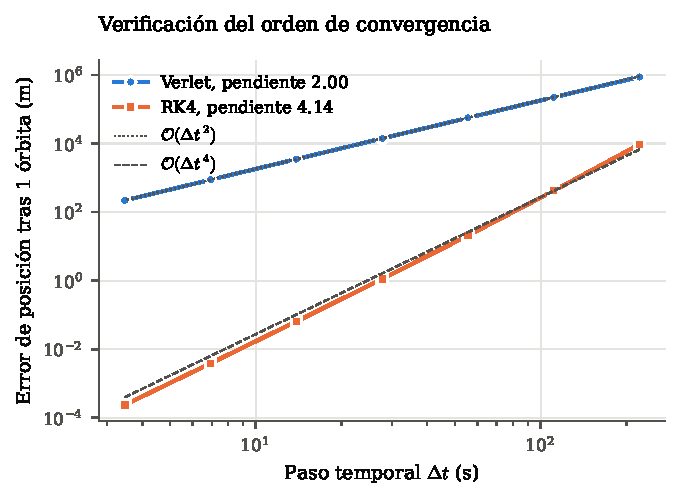
\includegraphics[width=0.62\textwidth]{fig04_orden_convergencia.pdf}
\caption{Error de posición tras una órbita frente al paso temporal. Las pendientes ajustadas coinciden con los órdenes teóricos.}
\label{fig:orden}
\end{figure}

%==========================================================================
\section{Resultados y discusión}
%==========================================================================
\subsection{Ascenso atmosférico}
La \autoref{fig:ascenso} muestra el perfil de ascenso y la \autoref{tab:asc} resume los eventos. El vehículo supera Mach~1 a los \RTMachOneS~\si{s} ($h=\RHMachOneKm~\si{km}$) y alcanza Max-Q de \RMaxqKpa~\si{kPa} a los \RTMaxqS~\si{s} ($h=\RHMaxqKm~\si{km}$, $M=\RMachMaxq$), valores del mismo orden que los publicados para el SLS (unos \SI{30}{kPa}). Max-Q ocurre en régimen supersónico bajo porque $q=\tfrac12\rho v^2$ resulta de competir entre el aumento de $v$ y la caída exponencial de $\rho$. En la separación de los SRB ($t=\RTSrbSepS~\si{s}$, $h=\RHSrbSepKm~\si{km}$) la masa salta en las \SI{199.6}{t} de estructura descartada y la aceleración sensada cae de forma abrupta. Durante la fase de la etapa central, la aceleración crece como $T/m(t)$ y alcanza \RMaxG\,$g_0$ en el MECO; el vehículo real limita este valor estrangulando los RS-25, un efecto no modelado aquí.

\begin{figure}[p]
\centering
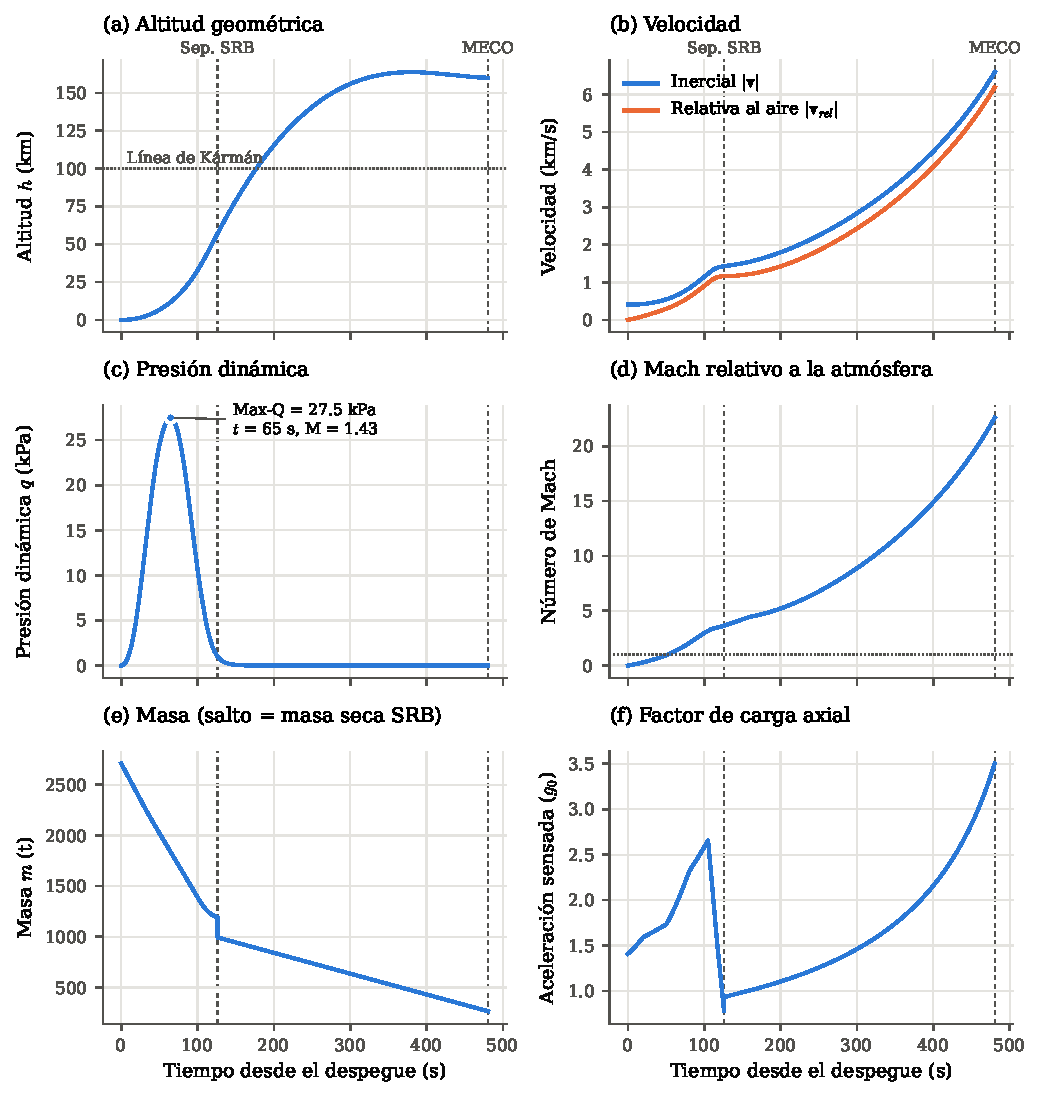
\includegraphics[width=\textwidth]{fig01_ascenso_perfil.pdf}
\caption{Perfil de ascenso del SLS Block~1B desde el LC-39B. Las líneas discontinuas marcan la separación de los SRB y el MECO. (a) Altitud; (b) velocidad inercial y relativa al aire, cuya diferencia inicial de unos \SI{408}{m/s} se debe a la rotación terrestre; (c) presión dinámica con Max-Q; (d) número de Mach; (e) masa; (f) aceleración no gravitacional en unidades de $g_0$.}
\label{fig:ascenso}
\end{figure}

\begin{figure}[ht]
\centering
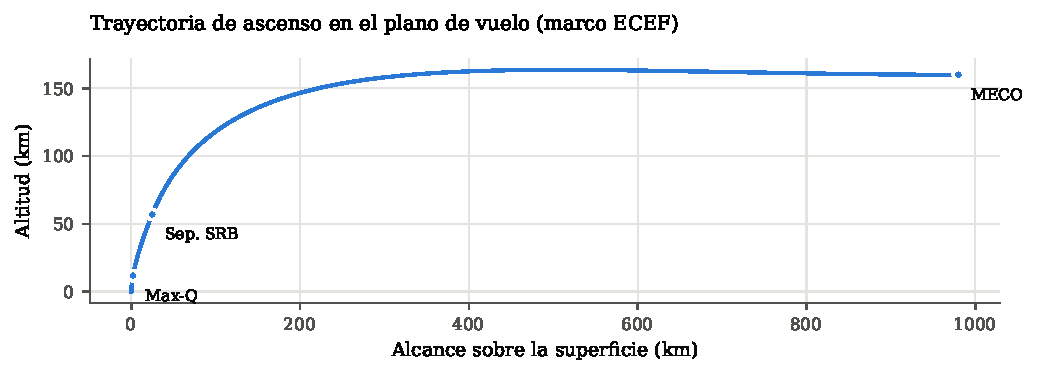
\includegraphics[width=\textwidth]{fig02_ascenso_trayectoria.pdf}
\caption{Altitud frente a alcance sobre la superficie (en el marco terrestre rotante) hasta el MECO.}
\label{fig:asc_traj}
\end{figure}

\begin{table}[ht]
\centering
\caption{Eventos del ascenso nominal simulado.}
\label{tab:asc}
\small
\begin{tabular}{@{}lrrr@{}}
\toprule
\textbf{Evento} & $t$ (s) & $h$ (km) & Magnitud \\
\midrule
Mach 1 & \RTMachOneS & \RHMachOneKm & -- \\
Max-Q & \RTMaxqS & \RHMaxqKm & $q=\RMaxqKpa~\si{kPa}$ \\
Separación SRB & \RTSrbSepS & \RHSrbSepKm & $v=\RVSrbSepKms~\si{km/s}$ \\
MECO & \RTMecoS & \RHMecoKm & $v=\RVMecoKms~\si{km/s}$, $\gamma=\ang{\RFpaMecoDeg}$ \\
\bottomrule
\end{tabular}
\end{table}

\paragraph{Presupuesto de la EUS.} En el MECO, la velocidad inercial (\RVMecoKms~\si{km/s}) es inferior a la circular a \SI{160}{km} (\RVCircMecoKms~\si{km/s}): la etapa central del Block~1B deja el vehículo en una trayectoria suborbital y la EUS debe completar la inserción con $\Delta v\approx\RDvInsertionKms~\si{km/s}$. Con la ecuación de Tsiolkovsky, la EUS cargada con \REusPayloadT~\si{t} de carga útil dispone de $\Delta v_{EUS}=I_{sp}g_0\ln(m_0/m_f)=\RDvEusTotalKms~\si{km/s}$. Tras la inserción y la TLI calculada (\autoref{sec:tli}) quedan unas \REusPropRemainingT~\si{t} de propelente, lo que muestra que la misión es factible dentro del modelo impulsivo (sin pérdidas por gravedad durante las combustiones finitas).

\subsection{Comparación de integradores en el régimen conservativo}
La \autoref{fig:conserv} compara Verlet, RK4 y DOP853 durante \RNOrbitsCmp{} órbitas a \SI{400}{km}, con \RStepsPerOrbitCmp{} pasos por órbita para los métodos de paso fijo. Pese a ser de menor orden, el error de energía de Verlet oscila sin crecer (máximo \RVerletMaxDe), en concordancia con la conservación del hamiltoniano modificado. El de RK4 crece monótonamente hasta \RRkFourFinalDe{}, una disipación numérica que se traduce en un decaimiento artificial de la órbita. Verlet conserva el momento angular hasta el redondeo (\RVerletMaxDh). DOP853 con tolerancias estrictas logra errores menores (\RDopEightFiveThreeFinalDe), pero también muestra deriva lineal y requiere muchas más evaluaciones de fuerza. Para propagaciones largas con un presupuesto de cómputo fijo, el integrador simpléctico ofrece el comportamiento cualitativo correcto.

\begin{figure}[ht]
\centering
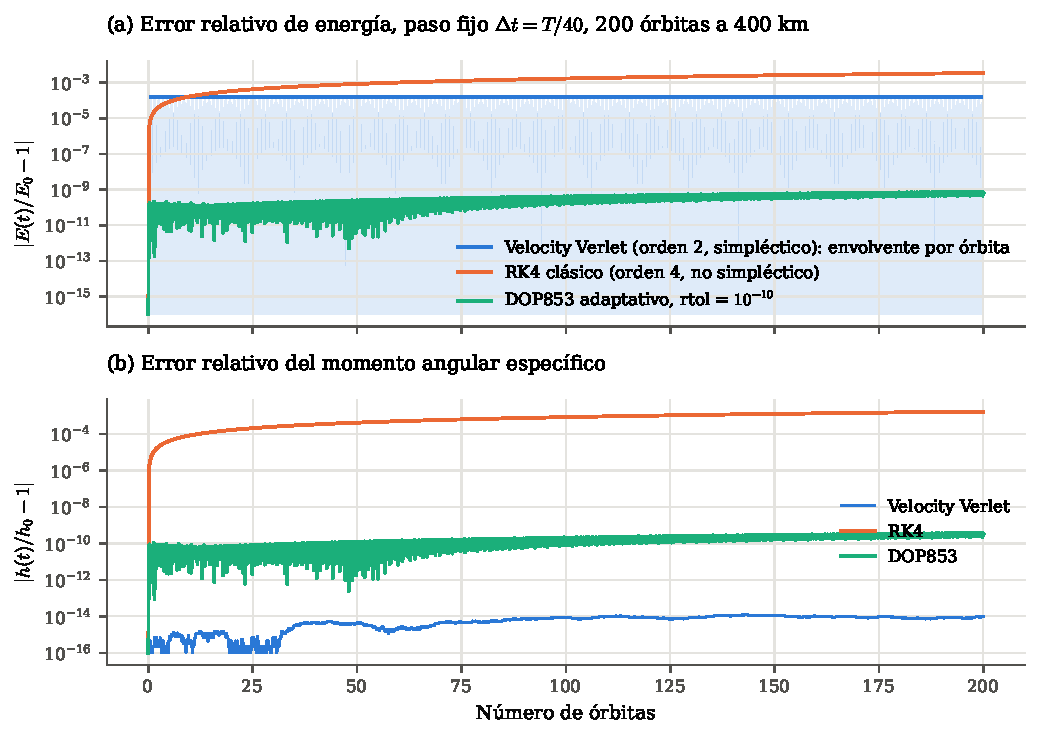
\includegraphics[width=\textwidth]{fig03_conservacion_integradores.pdf}
\caption{Errores relativos de energía (a) y momento angular (b) en el problema de Kepler. Verlet: envolvente por órbita (línea) y oscilación instantánea (sombreado).}
\label{fig:conserv}
\end{figure}

\subsection{Inyección translunar}\label{sec:tli}
Desde una órbita circular de aparcamiento a \RHParkKm~\si{km}, el método del disparo converge en \RTliIterations{} iteraciones a $|\Delta\vect v|=\RTliDvMs~\si{m/s}$ con un residuo de \RTliFinalResidualM~m (\autoref{fig:shoot}). La convergencia es cuadrática en las últimas iteraciones, como corresponde a Newton cerca de la raíz, y $\kappa(J)\le\RCondMax$ indica un problema bien condicionado. El $\Delta v$ obtenido coincide con el valor clásico de una TLI (de \num{3.1} a \SI{3.2}{km/s}~\cite{curtis2013}) y difiere solo en \SI{4}{m/s} de la semilla kepleriana: la Luna modifica sobre todo la \emph{dirección} de llegada, no la energía requerida. Repropagada con Verlet ($\Delta t=\SI{1}{s}$), la trayectoria llega a \RVerletArrivalAltKm~\si{km} de altitud lunar, a \RVerletTargetMissKm~\si{km} del objetivo calculado con DOP853. Esta discrepancia corresponde al error de discretización de orden 2 amplificado por el encuentro hiperbólico.

\begin{figure}[ht]
\centering
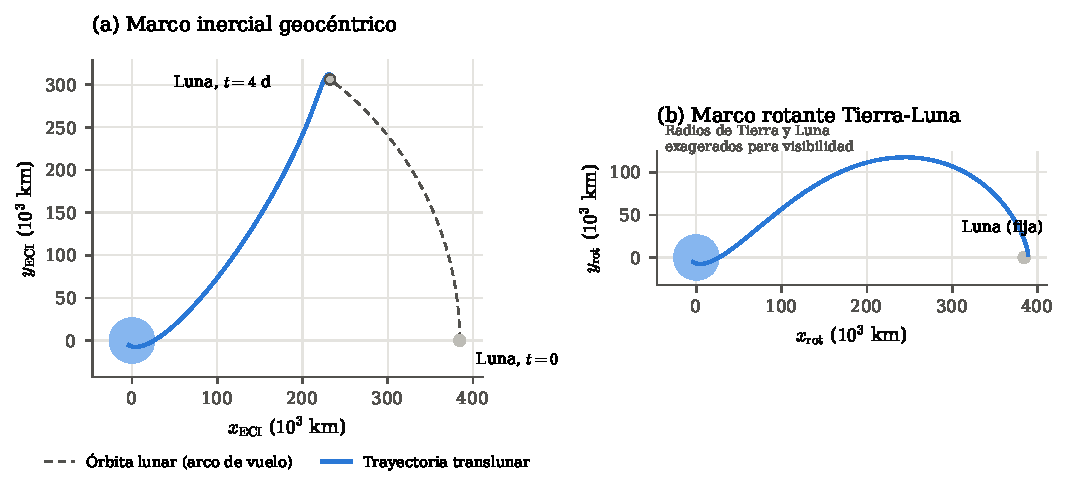
\includegraphics[width=\textwidth]{fig05_trayectoria_tli.pdf}
\caption{Trayectoria translunar de \RTliFlightDays{} días en el marco inercial (a) y en el marco rotante Tierra--Luna (b). En (b) la Luna permanece fija sobre el eje $x$.}
\label{fig:tli}
\end{figure}

\begin{figure}[ht]
\centering
\begin{subfigure}[b]{0.45\textwidth}
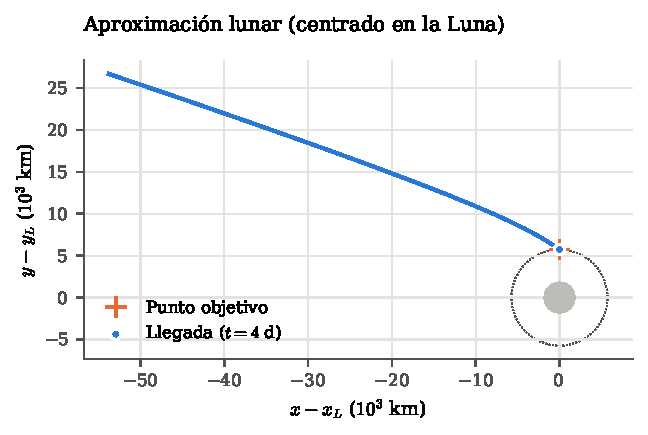
\includegraphics[width=\textwidth]{fig06_encuentro_lunar.pdf}
\caption{Aproximación selenocéntrica; el círculo punteado marca \RTliFlybyAltKm~\si{km} de altitud.}
\end{subfigure}\hfill
\begin{subfigure}[b]{0.53\textwidth}
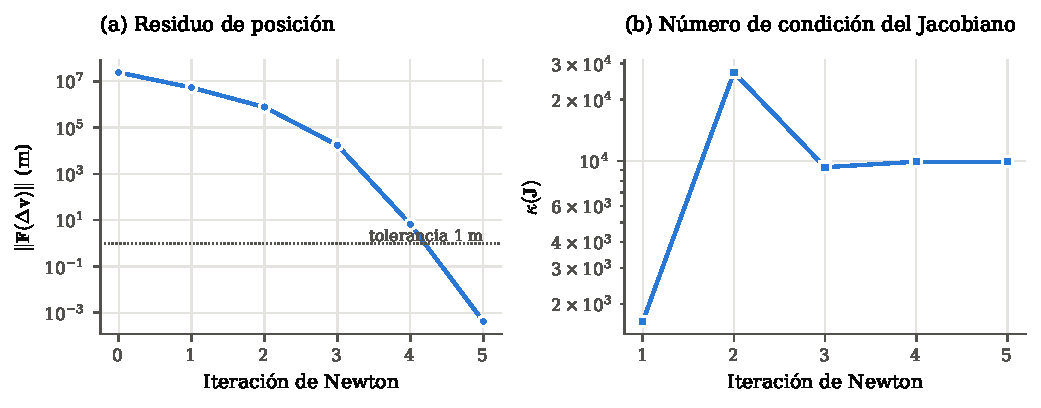
\includegraphics[width=\textwidth]{fig07_convergencia_disparo.pdf}
\caption{Residuo y número de condición en cada iteración de Newton.}
\end{subfigure}
\caption{Llegada a la Luna y convergencia del método del disparo.}
\label{fig:shoot}
\end{figure}

\subsection{Invariante de Jacobi}
La \autoref{fig:jacobi} contrasta la energía geocéntrica, que varía un \RGeoEnergyMaxRel{} durante el encuentro lunar porque no es una constante del movimiento, con la integral de Jacobi, cuyo error relativo se mantiene en \RJacobiMaxRel. El error de $E_J$ se acumula casi por completo en la primera hora, cuando el vehículo está cerca del perigeo y el paso de \SI{1}{s} es menos pequeño frente a la escala de tiempo local. Después permanece constante, la firma del hamiltoniano modificado de un integrador simpléctico.

\begin{figure}[ht]
\centering
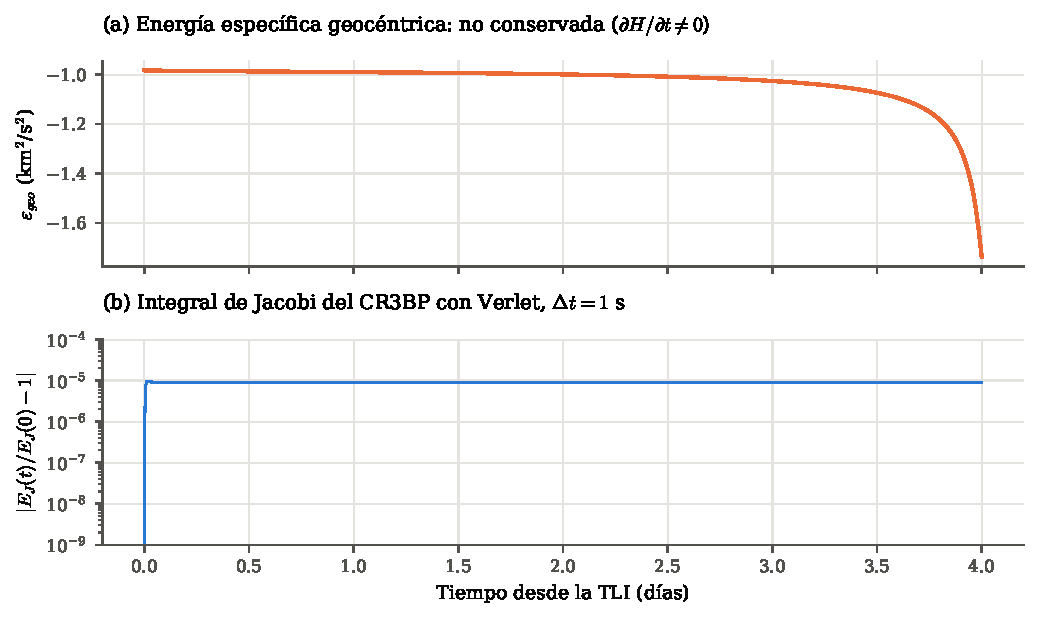
\includegraphics[width=\textwidth]{fig08_jacobi.pdf}
\caption{(a) Energía específica geocéntrica durante el tránsito; (b) error relativo de la integral de Jacobi con Verlet.}
\label{fig:jacobi}
\end{figure}

%==========================================================================
\section{Limitaciones}
%==========================================================================
\begin{itemize}
  \item Tierra esférica sin $J_2$, atmósfera exponencial sin viento, ángulo de ataque nulo y sin estrangulamiento de los RS-25.
  \item Plataforma de lanzamiento situada en el meridiano de referencia del ECI en $t=0$ (sin tiempo sidéreo de Greenwich) y TLI desde una órbita ecuatorial coplanar con la Luna. La inclinación real de la órbita de aparcamiento (de unos \ang{28.5}) y la de la órbita lunar (entre \ang{18.3} y \ang{28.6} respecto al ecuador) no se modelan.
  \item TLI impulsiva; la combustión real de la EUS dura varios minutos y tiene pérdidas por gravedad.
  \item Órbita lunar circular sin perturbación solar (modelo CR3BP).
\end{itemize}

%==========================================================================
\section{Conclusiones y trabajo futuro}\label{sec:futuro}
%==========================================================================
Se desarrolló y verificó un simulador modular de las fases de ascenso y tránsito translunar de Artemis~IV. La revisión física corrigió errores de conservación de masa, de consistencia del modelo de tres cuerpos y de formulación en el documento. Los resultados numéricos (Max-Q $\approx\RMaxqKpa~\si{kPa}$, MECO suborbital a \RHMecoKm~\si{km} y TLI de \RTliDvMs~\si{m/s}) son coherentes con los valores publicados para el SLS. Se comprobó cuantitativamente la ventaja cualitativa de los integradores simplécticos: el error de energía permanece acotado frente a la deriva secular de RK4. También se mostró que, con la Luna activa, el invariante correcto es la integral de Jacobi y no la energía geocéntrica. Por último, una buena semilla (la solución de la ecuación de Kepler) es determinante para la convergencia del método del disparo.

Como trabajo futuro se proponen:
\begin{enumerate}
  \item \textbf{Inserción en la NRHO:} generar la familia de órbitas de halo L2 sur en el CR3BP por corrección diferencial y continuación, y calcular el $\Delta v$ de inserción~\cite{howell2001,zimovan2017}.
  \item \textbf{Descenso lunar del HLS} con el potencial gravitatorio en armónicos esféricos,
  \begin{equation}
  U=\frac{\mu_L}{r}\left[1+\sum_{n=2}^{N}\sum_{m=0}^{n}\left(\frac{R_L}{r}\right)^n\bar P_{nm}(\sin\phi)\left(\bar C_{nm}\cos m\lambda+\bar S_{nm}\sin m\lambda\right)\right],
  \end{equation}
  con los coeficientes GRGM1200A de GRAIL~\cite{zuber2013,goossens2016}, $\phi$ la latitud y $\lambda$ la longitud selenocéntricas, y un integrador adaptativo con empuje variable.
  \item Efemérides JPL DE440 (SPICE), perturbación solar, $J_2$ terrestre y presión de radiación solar.
  \item Combustiones finitas de la EUS y optimización conjunta de la trayectoria de ascenso.
  \item Exportación de las trayectorias a la visualización WebGL/Three.js del repositorio.
\end{enumerate}

%==========================================================================
\begin{thebibliography}{99}
\bibitem{nasa2020artemis} NASA (2020). \textit{Artemis Plan: NASA's Lunar Exploration Program Overview}. National Aeronautics and Space Administration, Washington, DC.
\bibitem{nasa2023slsfacts} NASA (2023). \textit{Space Launch System Fact Sheet} (FS-2023-06-0080-MSFC). Marshall Space Flight Center.
\bibitem{nasa2018slslift} NASA (2018). \textit{Space Launch System Lift Capabilities and Configurations}. Marshall Space Flight Center.
\bibitem{sutton2017} Sutton, G.~P., \& Biblarz, O. (2017). \textit{Rocket Propulsion Elements} (9th ed.). Wiley.
\bibitem{curtis2013} Curtis, H.~D. (2013). \textit{Orbital Mechanics for Engineering Students} (3rd ed.). Butterworth-Heinemann.
\bibitem{szebehely1967} Szebehely, V. (1967). \textit{Theory of Orbits: The Restricted Problem of Three Bodies}. Academic Press.
\bibitem{hairer2006} Hairer, E., Lubich, C., \& Wanner, G. (2006). \textit{Geometric Numerical Integration: Structure-Preserving Algorithms for Ordinary Differential Equations} (2nd ed.). Springer.
\bibitem{dormand1980} Dormand, J.~R., \& Prince, P.~J. (1980). A family of embedded Runge--Kutta formulae. \textit{Journal of Computational and Applied Mathematics}, 6(1), 19--26.
\bibitem{howell2001} Howell, K.~C. (2001). Families of orbits in the vicinity of the collinear libration points. \textit{The Journal of the Astronautical Sciences}, 49(1), 107--125.
\bibitem{zimovan2017} Zimovan, E.~M., Howell, K.~C., \& Davis, D.~C. (2017). Near rectilinear halo orbits and their application in cis-lunar space. \textit{3rd IAA Conference on Dynamics and Control of Space Systems}, Moscú.
\bibitem{zuber2013} Zuber, M.~T., et al. (2013). Gravity field of the Moon from the Gravity Recovery and Interior Laboratory (GRAIL) mission. \textit{Science}, 339(6120), 668--671.
\bibitem{goossens2016} Goossens, S., et al. (2016). A global degree and order 1200 model of the lunar gravity field using GRAIL mission data. \textit{47th Lunar and Planetary Science Conference}, Abstract 1484.
\bibitem{nasa1976std} NOAA, NASA, USAF (1976). \textit{U.S. Standard Atmosphere, 1976}. U.S. Government Printing Office, Washington, DC.
\end{thebibliography}

\appendix
\section{Arquitectura del código y reproducibilidad}
\begin{tabularx}{\textwidth}{@{}lX@{}}
\toprule
\textbf{Módulo} & \textbf{Contenido} \\
\midrule
\texttt{constants.py} & Cuerpos celestes, rotación terrestre y etapas del SLS Block~1B. \\
\texttt{state.py} & Vector de estado inmutable $[\vect r,\vect v,m]$ validado. \\
\texttt{physics\_engine.py} & Gravedad, atmósfera US76, Mach, $C_D(M)$, arrastre, empuje y gasto másico. \\
\texttt{ascent\_solver.py} & Ecuaciones del ascenso, perfil SRB, guiado, eventos y \texttt{simulate\_full\_ascent}. \\
\texttt{ephemeris.py} & Órbita lunar circular con $n$ kepleriano. \\
\texttt{symplectic\_solver.py} & Fuerzas del CR3BP, Verlet, RK4, DOP853, energía e integral de Jacobi. \\
\texttt{shooting\_method.py} & Disparo, jacobiano numérico, Newton amortiguado y geometría kepleriana. \\
\texttt{scripts/generate\_figures.py} & Genera todas las figuras y \texttt{results.tex}. \\
\bottomrule
\end{tabularx}

\medskip\noindent
Todos los valores numéricos del texto se insertan automáticamente desde \texttt{results.tex}. Para reproducirlos:
\begin{verbatim}
python -m pytest                      # 63 pruebas
python scripts/generate_figures.py    # figuras + results.tex
cd docs/paper/final && pdflatex main.tex && pdflatex main.tex
\end{verbatim}

\end{document}
